\input /Users/davidmcallester/Icloude/tex/SlidePreamble
\input /Users/davidmcallester/Icloude/tex/preamble


\begin{document}

{\Huge
  \centerline{\bf TTIC 31230,  Fundamentals of Deep Learning}
  \vfill
  \centerline{David McAllester, Autumn 2020}
  \vfill
  \centerline{\bf  The Transformer Part I}
  \vfill
  \vfill

\slide{The Transformer}

Attention is All You Need, Vaswani et al., June 2017

\vfill
The Transformer has now essentially replaced RNNs in natural language applications.

\vfill

The recent progress on the natural language understanding evaluation (GLUE) is based on general language modeling using Transformers.

\slide{Vector Sequences}

\vfill
Each layer in the Transformer has shape $L[T,J]$ where $t$ ranges over the position in the input sequence and $j$ ranges over neurons at that position
(and omitting the batch index).

\vfill
This is the same shape as layers in an RNN --- a sequence of vectors $L[t,J]$.

\vfill
When processing sentences, $T$ is the sentence length.

\slide{Parallel Layer Computation}

However, in the Transformer we can compute the layer $L_{\ell+1}[T,J]$ from $L_\ell[T,J]$ in $O(\ln T)$ time (in parallel).

\vfill
The log comes from the time to compute a large sum in parallel using a tree of additions.

\vfill
This is an important difference from RNNs which compute sequentially over time.

\vfill
In this respect the Transformer is more similar to a CNN than to an RNN.

\slide{Self-Attention}

The fundamental innovation of the Transformer is the self-attention layer.

\vfill
For each position $t$ in the sequence we compute an attention over the other positions in the sequence.

\vfill
These attentions can be viewed as a soft directed graph over the positions where
the attention from $t_1$ to $t_2$ can be viewed as a weighted directed edge from position $t_1$ to position $t_2$.

\vfill
There is an intuitive analogy between this soft graph and a dependency parse tree.

\slide{Transformer Heads}

In a dependency parse edges are typically labeled with grammatical roles such as ``subject-of'' or ``object-of''.

\vfill
The self attention layers of the Transformer we have ``heads'' which can be viewed as labels for dependency edges.

\vfill
Self attention constructs a tensor $\alpha[k,t_1,t_2]$ --- the strength of the attention weight (edge weight)
from $t_1$ to $t_2$ with head (label) $k$.

\slide{Query-Key Attention}

For each head $k$ and position $t$ we compute a key vector and a query vector with dimension $I$ typically smaller than dimension $J$.

\begin{eqnarray*}
\mathrm{Query}_{\ell+1}[k,t,i] & = & W^Q_{\ell+1}[k,i,J]L_\ell[t,J] \\
\\
\mathrm{Key}_{\ell+1}[k,t,i] & = &  W^K_{\ell+1}[k,i,J]L_\ell[t,J] \\
\\
\alpha_{\ell+1}[k,t_1,t_2] & = & \softmax_{t_2}\; \frac{1}{\sqrt{I}}\;\mathrm{Query}_{\ell+1}[k,t_1,I]\mathrm{Key}_{\ell+1}[k,t_2,I]
\end{eqnarray*}

\slide{Computing the Output}
      
\begin{eqnarray*}
\mathrm{Value}_{\ell+1}[k,t,i] & = & W^V_{\ell+1}[k,i,J]L_\ell[t,J] \\
\\
h^1_{\ell+1}[k,t,i] & = & \alpha[k,t,T]\mathrm{Value}[k,T,i] \\
\\
h^2_{\ell+1}[t,C] & = & h^1_{\ell+1}[0,t,I];\cdots;h^1_{\ell+1}[K-1,t,I] \\
\\
L_{\ell+1}[t,j] & = & W^0_{\ell+1}[j,C]h^2[t,C]
\end{eqnarray*}

\vfill
Here semicolon denotes vector concatenation.

\slide{The Transformer Layer}

Each ``Transformer layer'' consists of six ``sublayers'' the first of which is the self-attention.


\centerline{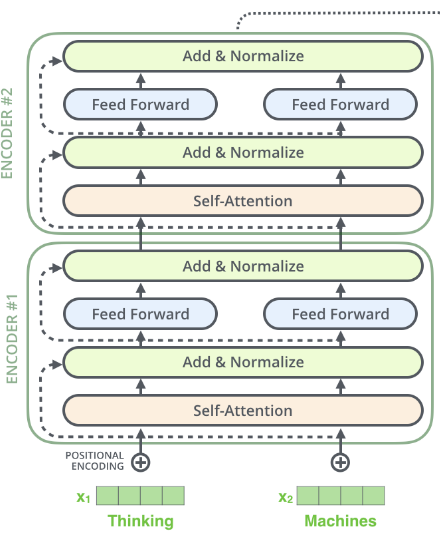
\includegraphics[height=3.5in]{\images/transformer}}

{\Large
\centerline{Jay Alammar's blog}
}

The other layers are discussed in the next unit.

\slide{END}

}
\end{document}
